\documentclass[tikz,border=4pt]{standalone}
\usepackage{tikz}
\usepackage{xcolor}
\usepackage{amsmath}

\definecolor{mleblue}{HTML}{2A78D6}
\definecolor{mleorange}{HTML}{EB6834}
\definecolor{mlegray}{HTML}{C3C2B7}
\definecolor{mleink}{HTML}{0B0B0B}
\definecolor{mlesub}{HTML}{52514E}
\definecolor{mlemut}{HTML}{898781}
\definecolor{mlegrid}{HTML}{E1E0D9}
\definecolor{mlesurf}{HTML}{FCFCFB}

\begin{document}
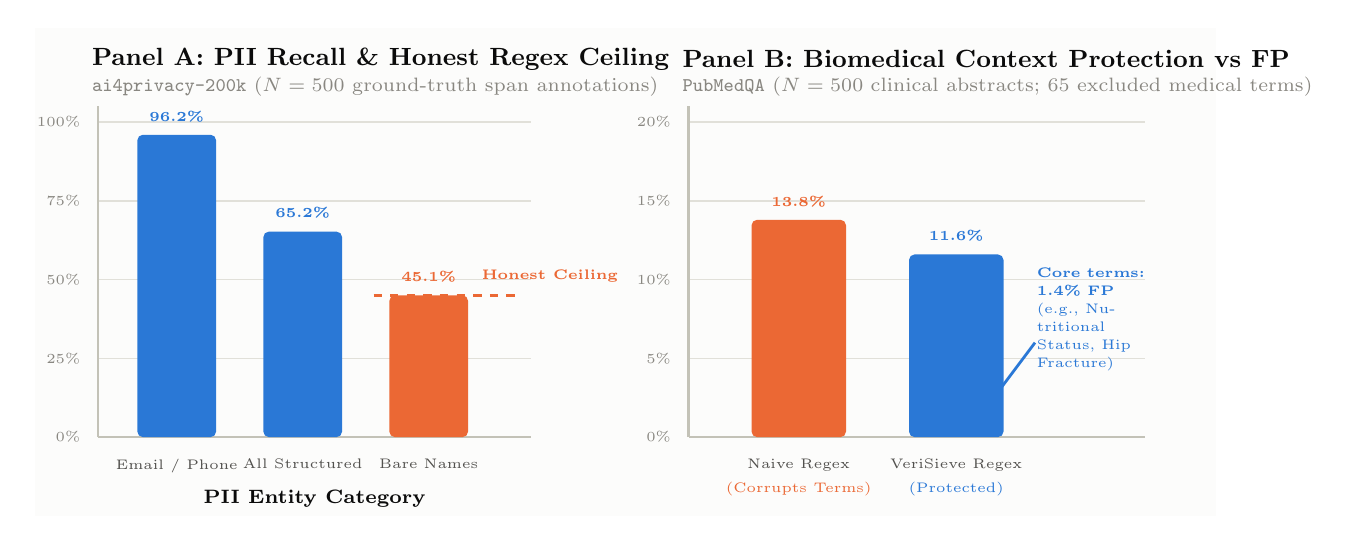
\begin{tikzpicture}[x=1cm, y=1cm, font=\sffamily]
  % Background surface
  \fill[mlesurf] (-0.8, -1.0) rectangle (14.2, 5.2);

  % ================= PANEL A =================
  \begin{scope}[shift={(0,0)}]
    \node[anchor=west, text=mleink, font=\bfseries\small] at (-0.2, 4.8) {Panel A: PII Recall \& Honest Regex Ceiling};
    \node[anchor=west, text=mlemut, font=\scriptsize] at (-0.2, 4.45) {\texttt{ai4privacy-200k} ($N=500$ ground-truth span annotations)};

    % Grid lines
    \draw[mlegrid, line width=0.5pt] (0,0) -- (5.5,0);
    \draw[mlegrid, line width=0.5pt] (0,1.0) -- (5.5,1.0);
    \draw[mlegrid, line width=0.5pt] (0,2.0) -- (5.5,2.0);
    \draw[mlegrid, line width=0.5pt] (0,3.0) -- (5.5,3.0);
    \draw[mlegrid, line width=0.5pt] (0,4.0) -- (5.5,4.0);

    % Y Axis labels
    \node[anchor=east, text=mlemut, font=\tiny] at (-0.1, 0) {0\%};
    \node[anchor=east, text=mlemut, font=\tiny] at (-0.1, 1.0) {25\%};
    \node[anchor=east, text=mlemut, font=\tiny] at (-0.1, 2.0) {50\%};
    \node[anchor=east, text=mlemut, font=\tiny] at (-0.1, 3.0) {75\%};
    \node[anchor=east, text=mlemut, font=\tiny] at (-0.1, 4.0) {100\%};

    % Axes
    \draw[mlegray, line width=0.8pt] (0,0) -- (5.5,0);
    \draw[mlegray, line width=0.8pt] (0,0) -- (0,4.2);

    % Bar 1: Email / Phone / IP (High Structured Recall >95%)
    \fill[mleblue, rounded corners=2pt] (0.5, 0) rectangle (1.5, 3.84);
    \node[anchor=south, text=mleblue, font=\tiny\bfseries] at (1.0, 3.88) {96.2\%};
    \node[anchor=north, text=mlesub, font=\tiny] at (1.0, -0.15) {Email / Phone};

    % Bar 2: Structured Overall
    \fill[mleblue, rounded corners=2pt] (2.1, 0) rectangle (3.1, 2.61);
    \node[anchor=south, text=mleblue, font=\tiny\bfseries] at (2.6, 2.65) {65.2\%};
    \node[anchor=north, text=mlesub, font=\tiny] at (2.6, -0.15) {All Structured};

    % Bar 3: Unstructured Bare Names (Ceiling!)
    \fill[mleorange, rounded corners=2pt] (3.7, 0) rectangle (4.7, 1.80);
    \node[anchor=south, text=mleorange, font=\tiny\bfseries] at (4.2, 1.84) {45.1\%};
    \node[anchor=north, text=mlesub, font=\tiny] at (4.2, -0.15) {Bare Names};

    % Ceiling indicator line
    \draw[mleorange, dashed, line width=1.0pt] (3.5, 1.80) -- (5.3, 1.80);
    \node[anchor=west, text=mleorange, font=\fontsize{5}{6}\selectfont] at (4.75, 2.05) {\textbf{Honest Ceiling}};

    \node[anchor=north, text=mleink, font=\scriptsize\bfseries] at (2.75, -0.55) {PII Entity Category};
  \end{scope}

  % ================= PANEL B =================
  \begin{scope}[shift={(7.5,0)}]
    \node[anchor=west, text=mleink, font=\bfseries\small] at (-0.2, 4.8) {Panel B: Biomedical Context Protection vs FP};
    \node[anchor=west, text=mlemut, font=\scriptsize] at (-0.2, 4.45) {\texttt{PubMedQA} ($N=500$ clinical abstracts; 65 excluded medical terms)};

    % Grid lines
    \draw[mlegrid, line width=0.5pt] (0,0) -- (5.8,0);
    \draw[mlegrid, line width=0.5pt] (0,1.0) -- (5.8,1.0);
    \draw[mlegrid, line width=0.5pt] (0,2.0) -- (5.8,2.0);
    \draw[mlegrid, line width=0.5pt] (0,3.0) -- (5.8,3.0);
    \draw[mlegrid, line width=0.5pt] (0,4.0) -- (5.8,4.0);

    % Y Axis labels
    \node[anchor=east, text=mlemut, font=\tiny] at (-0.1, 0) {0\%};
    \node[anchor=east, text=mlemut, font=\tiny] at (-0.1, 1.0) {5\%};
    \node[anchor=east, text=mlemut, font=\tiny] at (-0.1, 2.0) {10\%};
    \node[anchor=east, text=mlemut, font=\tiny] at (-0.1, 3.0) {15\%};
    \node[anchor=east, text=mlemut, font=\tiny] at (-0.1, 4.0) {20\%};

    % Axes
    \draw[mlegray, line width=0.8pt] (0,0) -- (5.8,0);
    \draw[mlegray, line width=0.8pt] (0,0) -- (0,4.2);

    % Bar 1: Naive Title-Case Regex FP (13.8% across full text, >80% on clinical terms)
    \fill[mleorange, rounded corners=2pt] (0.8, 0) rectangle (2.0, 2.76);
    \node[anchor=south, text=mleorange, font=\tiny\bfseries] at (1.4, 2.80) {13.8\%};
    \node[anchor=north, text=mlesub, font=\tiny] at (1.4, -0.15) {Naive Regex};
    \node[anchor=north, text=mleorange, font=\fontsize{5}{6}\selectfont] at (1.4, -0.45) {(Corrupts Terms)};

    % Bar 2: VeriSieve with Domain Exclusions
    \fill[mleblue, rounded corners=2pt] (2.8, 0) rectangle (4.0, 2.32);
    \node[anchor=south, text=mleblue, font=\tiny\bfseries] at (3.4, 2.36) {11.6\%};
    \node[anchor=north, text=mlesub, font=\tiny] at (3.4, -0.15) {VeriSieve Regex};
    \node[anchor=north, text=mleblue, font=\fontsize{5}{6}\selectfont] at (3.4, -0.45) {(Protected)};

    % Annotation on Core Clinical Nouns (1.4% FP)
    \draw[mleblue, line width=1.0pt, ->] (4.4, 1.2) -- (3.8, 0.4);
    \node[anchor=west, text=mleblue, font=\fontsize{5.5}{6.5}\selectfont, text width=1.4cm] at (4.3, 1.5) {\textbf{Core terms: 1.4\% FP} (e.g., Nutritional Status, Hip Fracture)};
  \end{scope}
\end{tikzpicture}
\end{document}
